% F. J. Marshall - J. R. Capablanca, New York, 1918, with Capablanca's notes.
% Build with: python3 ../../tools/chessbook.py game-14-marshall-capablanca.tex
\documentclass[10pt,twoside]{article}
\usepackage[paperwidth=487.56bp,paperheight=691.65bp,top=72pt,bottom=44pt,inner=50pt,outer=48pt,
            headheight=13pt,headsep=20pt,footskip=0pt]{geometry}
\usepackage[T1]{fontenc}
\usepackage[lining]{ebgaramond}
\usepackage{graphicx}
\usepackage{microtype}
\usepackage{tikz}
\usepackage{fancyhdr}
\usepackage[hidelinks,pdftitle={Marshall - Capablanca, New York, 1918},
            pdfauthor={J. R. Capablanca}]{hyperref}

\newcommand{\textsizebook}{\fontsize{10.5}{12.6}\selectfont}
\AtBeginDocument{\textsizebook}
\setlength{\columnsep}{11pt}
\setlength{\parindent}{9pt}
\setlength{\parskip}{0pt}
\setlength{\emergencystretch}{1.5em}
\raggedbottom

\newlength{\boardwidth}
\setlength{\boardwidth}{160pt}

% A main line move, as a bold heading above its note
\newcommand{\Move}[1]{\par\addvspace{8pt}\noindent\phantomsection{\bfseries #1}\par\nopagebreak}
% A diagram in the text
\newcommand{\ChessDiagram}[1]{\par\addvspace{7pt}{\centering #1\par}\addvspace{5pt}}

\pagestyle{fancy}
\fancyhf{}
\renewcommand{\headrulewidth}{0pt}
\fancyhead[LE,RO]{\thepage}
\fancyhead[CE]{Queen's Gambit Declined}
\fancyhead[CO]{Marshall -- Capablanca}






\newcommand{\figK}{\raisebox{-0.14em}{
\includegraphics[height=1em]{diagrams/figK}}}
\newcommand{\figQ}{\raisebox{-0.14em}{
\includegraphics[height=1em]{diagrams/figQ}}}
\newcommand{\figR}{\raisebox{-0.14em}{
\includegraphics[height=1em]{diagrams/figR}}}
\newcommand{\figB}{\raisebox{-0.14em}{
\includegraphics[height=1em]{diagrams/figB}}}
\newcommand{\figN}{\raisebox{-0.14em}{
\includegraphics[height=1em]{diagrams/figN}}}
\begin{document}

\twocolumn[{%
\thispagestyle{empty}
\begin{tikzpicture}[remember picture,overlay]
  \node[circle,draw=black,line width=1.6pt,fill=black!20,minimum size=112pt] (seal)
       at ([xshift=75pt,yshift=-75pt]current page.north west) {};
  \draw[line width=0.9pt] ([shift={(-48pt,-30pt)}]seal.center) -- ([shift={(44pt,34pt)}]seal.center);
  \node[rotate=37] at ([shift={(-11pt,14pt)}]seal.center) {\fontsize{25}{25}\selectfont\bfseries Game};
  \node[rotate=37] at ([shift={(10pt,-16pt)}]seal.center) {\fontsize{38}{38}\selectfont\bfseries 14};
  \node[anchor=north east] at ([xshift=-14pt,yshift=-24pt]current page.north east)
       {\href{https://lichess.org/analysis/pgn/d4_d5_Nf3_Nf6_c4_e6_Nc3_Nbd7}{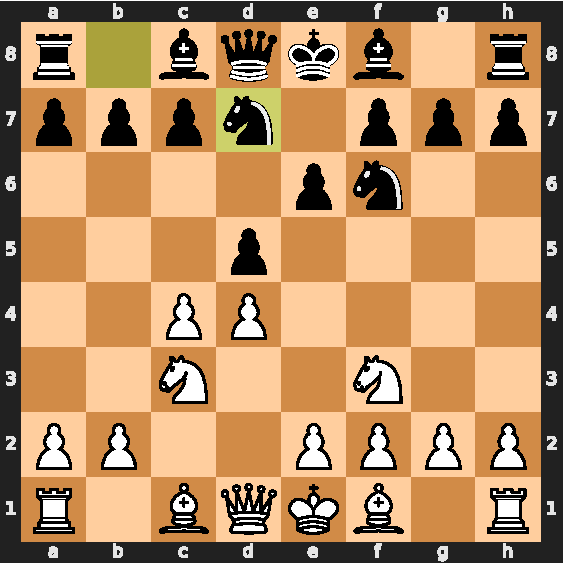
\includegraphics[width=108pt]{diagrams/board-adc6fe7accf7}}};
\end{tikzpicture}

\vspace*{38pt}
\begin{center}
  \begin{minipage}{235pt}\centering
    {\fontsize{22}{25}\selectfont\bfseries Queen's Gambit Declined\par}
    \vspace{4pt}\rule{\linewidth}{1pt}\\[-9.5pt]\rule{\linewidth}{0.4pt}
  \end{minipage}

  \vspace{14pt}
  {\fontsize{19}{22}\selectfont\bfseries Marshall -- Capablanca\par}
  \vspace{10pt}
  {\fontsize{15}{18}\selectfont\bfseries New York, 1918\par}
  \vspace{8pt}
  {\fontsize{11}{13}\selectfont White: F. J. Marshall \quad Black: J. R. Capablanca\par}
  \vspace{10pt}
  {\centering\fontsize{8.5}{10}\selectfont\itshape
   Notes by J. R. Capablanca, from \textup{Chess Fundamentals} (1921), which is in the public domain.\\
   Descriptive notation has been converted to algebraic. Page references are to the book.\\
   Click any move or diagram to open it on Lichess.\par}
\end{center}
\vspace{10pt}
}]
\textsizebook

\Move{\href{https://lichess.org/analysis/pgn/d4}{1.d4} \href{https://lichess.org/analysis/pgn/d4_d5}{d5} \href{https://lichess.org/analysis/pgn/d4_d5_Nf3}{2.\figN f3} \href{https://lichess.org/analysis/pgn/d4_d5_Nf3_Nf6}{\figN f6} \href{https://lichess.org/analysis/pgn/d4_d5_Nf3_Nf6_c4}{3.c4} \href{https://lichess.org/analysis/pgn/d4_d5_Nf3_Nf6_c4_e6}{e6} \href{https://lichess.org/analysis/pgn/d4_d5_Nf3_Nf6_c4_e6_Nc3}{4.\figN c3} \href{https://lichess.org/analysis/pgn/d4_d5_Nf3_Nf6_c4_e6_Nc3_Nbd7}{\figN bd7} \href{https://lichess.org/analysis/pgn/d4_d5_Nf3_Nf6_c4_e6_Nc3_Nbd7_Bg5}{5.\figB g5} \href{https://lichess.org/analysis/pgn/d4_d5_Nf3_Nf6_c4_e6_Nc3_Nbd7_Bg5_Be7}{\figB e7} \href{https://lichess.org/analysis/pgn/d4_d5_Nf3_Nf6_c4_e6_Nc3_Nbd7_Bg5_Be7_e3}{6.e3} \href{https://lichess.org/analysis/pgn/d4_d5_Nf3_Nf6_c4_e6_Nc3_Nbd7_Bg5_Be7_e3_O-O}{0--0} \href{https://lichess.org/analysis/pgn/d4_d5_Nf3_Nf6_c4_e6_Nc3_Nbd7_Bg5_Be7_e3_O-O_Rc1}{7.\figR c1} \href{https://lichess.org/analysis/pgn/d4_d5_Nf3_Nf6_c4_e6_Nc3_Nbd7_Bg5_Be7_e3_O-O_Rc1_c6}{c6}}

This is one of the oldest systems of defence against the Queen's Gambit. I had played it before in this Tournament against Kostic, and no doubt Marshall expected it. At times I change my defences, or rather systems of defence; on the other hand, during a Tournament, if one of them has given me good results, I generally play it all the time.

\Move{\href{https://lichess.org/analysis/pgn/d4_d5_Nf3_Nf6_c4_e6_Nc3_Nbd7_Bg5_Be7_e3_O-O_Rc1_c6_Qc2}{8.\figQ c2} \href{https://lichess.org/analysis/pgn/d4_d5_Nf3_Nf6_c4_e6_Nc3_Nbd7_Bg5_Be7_e3_O-O_Rc1_c6_Qc2_dxc4}{dxc4} \href{https://lichess.org/analysis/pgn/d4_d5_Nf3_Nf6_c4_e6_Nc3_Nbd7_Bg5_Be7_e3_O-O_Rc1_c6_Qc2_dxc4_Bxc4}{9.\figB xc4} \href{https://lichess.org/analysis/pgn/d4_d5_Nf3_Nf6_c4_e6_Nc3_Nbd7_Bg5_Be7_e3_O-O_Rc1_c6_Qc2_dxc4_Bxc4_Nd5}{\figN d5} \href{https://lichess.org/analysis/pgn/d4_d5_Nf3_Nf6_c4_e6_Nc3_Nbd7_Bg5_Be7_e3_O-O_Rc1_c6_Qc2_dxc4_Bxc4_Nd5_Bxe7}{10.\figB xe7} \href{https://lichess.org/analysis/pgn/d4_d5_Nf3_Nf6_c4_e6_Nc3_Nbd7_Bg5_Be7_e3_O-O_Rc1_c6_Qc2_dxc4_Bxc4_Nd5_Bxe7_Qxe7}{\figQ xe7} \href{https://lichess.org/analysis/pgn/d4_d5_Nf3_Nf6_c4_e6_Nc3_Nbd7_Bg5_Be7_e3_O-O_Rc1_c6_Qc2_dxc4_Bxc4_Nd5_Bxe7_Qxe7_O-O}{11.0--0} \href{https://lichess.org/analysis/pgn/d4_d5_Nf3_Nf6_c4_e6_Nc3_Nbd7_Bg5_Be7_e3_O-O_Rc1_c6_Qc2_dxc4_Bxc4_Nd5_Bxe7_Qxe7_O-O_Nxc3}{\figN xc3} \href{https://lichess.org/analysis/pgn/d4_d5_Nf3_Nf6_c4_e6_Nc3_Nbd7_Bg5_Be7_e3_O-O_Rc1_c6_Qc2_dxc4_Bxc4_Nd5_Bxe7_Qxe7_O-O_Nxc3_Qxc3}{12.\figQ xc3} \href{https://lichess.org/analysis/pgn/d4_d5_Nf3_Nf6_c4_e6_Nc3_Nbd7_Bg5_Be7_e3_O-O_Rc1_c6_Qc2_dxc4_Bxc4_Nd5_Bxe7_Qxe7_O-O_Nxc3_Qxc3_b6}{b6}}

This is the key to this system of defence. Having simplified the game considerably by a series of exchanges, Black will now develop his Queen's Bishop along the long diagonal without having created any apparent weakness. The proper development of the Queen's Bishop is Black's greatest problem in the Queen's Gambit.

\Move{\href{https://lichess.org/analysis/pgn/d4_d5_Nf3_Nf6_c4_e6_Nc3_Nbd7_Bg5_Be7_e3_O-O_Rc1_c6_Qc2_dxc4_Bxc4_Nd5_Bxe7_Qxe7_O-O_Nxc3_Qxc3_b6_e4}{13.e4} \href{https://lichess.org/analysis/pgn/d4_d5_Nf3_Nf6_c4_e6_Nc3_Nbd7_Bg5_Be7_e3_O-O_Rc1_c6_Qc2_dxc4_Bxc4_Nd5_Bxe7_Qxe7_O-O_Nxc3_Qxc3_b6_e4_Bb7}{\figB b7} \href{https://lichess.org/analysis/pgn/d4_d5_Nf3_Nf6_c4_e6_Nc3_Nbd7_Bg5_Be7_e3_O-O_Rc1_c6_Qc2_dxc4_Bxc4_Nd5_Bxe7_Qxe7_O-O_Nxc3_Qxc3_b6_e4_Bb7_Rfe1}{14.\figR fe1} \href{https://lichess.org/analysis/pgn/d4_d5_Nf3_Nf6_c4_e6_Nc3_Nbd7_Bg5_Be7_e3_O-O_Rc1_c6_Qc2_dxc4_Bxc4_Nd5_Bxe7_Qxe7_O-O_Nxc3_Qxc3_b6_e4_Bb7_Rfe1_Rfd8}{\figR fd8}}

\ChessDiagram{\href{https://lichess.org/analysis/pgn/d4_d5_Nf3_Nf6_c4_e6_Nc3_Nbd7_Bg5_Be7_e3_O-O_Rc1_c6_Qc2_dxc4_Bxc4_Nd5_Bxe7_Qxe7_O-O_Nxc3_Qxc3_b6_e4_Bb7_Rfe1_Rfd8}{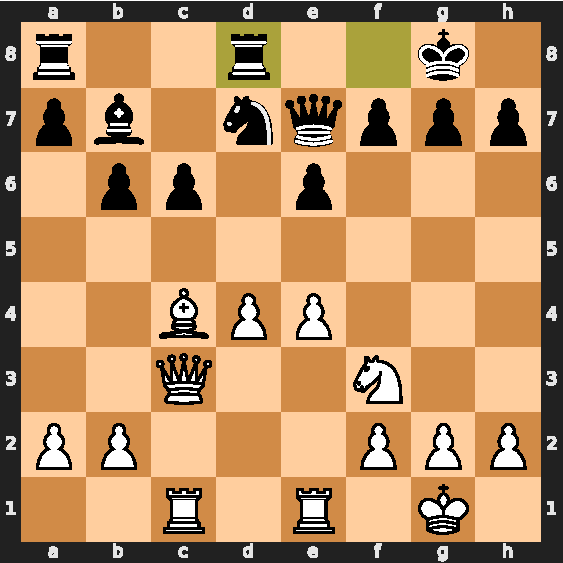
\includegraphics[width=\boardwidth]{diagrams/board-bec3bc7a375f}}}

The developing stage can now be said to be complete on both sides. The opening is over and the middle-game begins. White, as is generally the case, has obtained the centre. Black, on the other hand, is entrenched in his first three ranks, and if given time will post his Queen's Rook at c8 and his Knight at f6, and finally play ...c5, in order to break up White's centre and give full action to the Black Bishop posted at b7. In this game White attempts to anticipate that plan by initiating an advance on the centre, which, when carefully analysed, is truly an attack against Black's e-pawn.

\Move{\href{https://lichess.org/analysis/pgn/d4_d5_Nf3_Nf6_c4_e6_Nc3_Nbd7_Bg5_Be7_e3_O-O_Rc1_c6_Qc2_dxc4_Bxc4_Nd5_Bxe7_Qxe7_O-O_Nxc3_Qxc3_b6_e4_Bb7_Rfe1_Rfd8_d5}{15.d5} \href{https://lichess.org/analysis/pgn/d4_d5_Nf3_Nf6_c4_e6_Nc3_Nbd7_Bg5_Be7_e3_O-O_Rc1_c6_Qc2_dxc4_Bxc4_Nd5_Bxe7_Qxe7_O-O_Nxc3_Qxc3_b6_e4_Bb7_Rfe1_Rfd8_d5_Nc5}{\figN c5!}}

Against Kostic in a previous game I had played \href{https://lichess.org/analysis/pgn/d4_d5_Nf3_Nf6_c4_e6_Nc3_Nbd7_Bg5_Be7_e3_O-O_Rc1_c6_Qc2_dxc4_Bxc4_Nd5_Bxe7_Qxe7_O-O_Nxc3_Qxc3_b6_e4_Bb7_Rfe1_Rfd8_d5_Nf8}{15...\figN f8}. It was carelessness on my part, but Marshall believed differently, otherwise he would not have played this variation, since, had he analysed this move, he would, I think, have realised that Black would obtain an excellent game. Black now threatens not only ...cxd5; but also \figN xe4; followed by ...cxd5. The position is very interesting and full of possibilities.

\ChessDiagram{\href{https://lichess.org/analysis/pgn/d4_d5_Nf3_Nf6_c4_e6_Nc3_Nbd7_Bg5_Be7_e3_O-O_Rc1_c6_Qc2_dxc4_Bxc4_Nd5_Bxe7_Qxe7_O-O_Nxc3_Qxc3_b6_e4_Bb7_Rfe1_Rfd8_d5_Nc5}{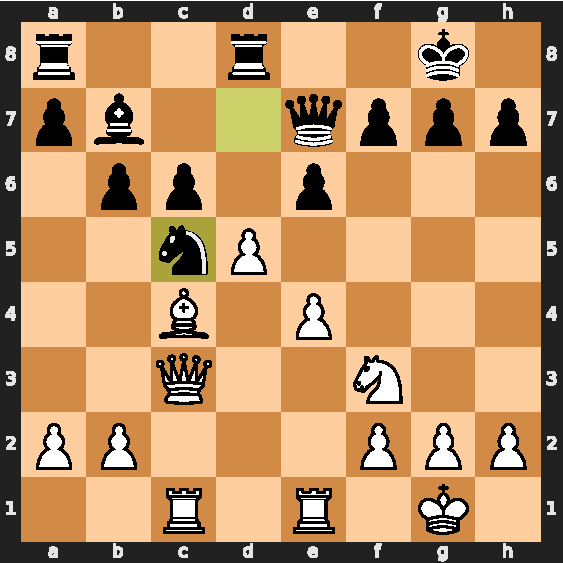
\includegraphics[width=\boardwidth]{diagrams/board-a16590bb1b2d}}}

\Move{\href{https://lichess.org/analysis/pgn/d4_d5_Nf3_Nf6_c4_e6_Nc3_Nbd7_Bg5_Be7_e3_O-O_Rc1_c6_Qc2_dxc4_Bxc4_Nd5_Bxe7_Qxe7_O-O_Nxc3_Qxc3_b6_e4_Bb7_Rfe1_Rfd8_d5_Nc5_dxe6}{16.dxe6} \href{https://lichess.org/analysis/pgn/d4_d5_Nf3_Nf6_c4_e6_Nc3_Nbd7_Bg5_Be7_e3_O-O_Rc1_c6_Qc2_dxc4_Bxc4_Nd5_Bxe7_Qxe7_O-O_Nxc3_Qxc3_b6_e4_Bb7_Rfe1_Rfd8_d5_Nc5_dxe6_Nxe6}{\figN xe6} \href{https://lichess.org/analysis/pgn/d4_d5_Nf3_Nf6_c4_e6_Nc3_Nbd7_Bg5_Be7_e3_O-O_Rc1_c6_Qc2_dxc4_Bxc4_Nd5_Bxe7_Qxe7_O-O_Nxc3_Qxc3_b6_e4_Bb7_Rfe1_Rfd8_d5_Nc5_dxe6_Nxe6_Bxe6}{17.\figB xe6} \href{https://lichess.org/analysis/pgn/d4_d5_Nf3_Nf6_c4_e6_Nc3_Nbd7_Bg5_Be7_e3_O-O_Rc1_c6_Qc2_dxc4_Bxc4_Nd5_Bxe7_Qxe7_O-O_Nxc3_Qxc3_b6_e4_Bb7_Rfe1_Rfd8_d5_Nc5_dxe6_Nxe6_Bxe6_Qxe6}{\figQ xe6}}

played under the impression that White had to lose time in defending his a-pawn, when I could play ...c5, obtaining a very superior game. But, as will be seen, my opponent had quite a little surprise for me.

\Move{\href{https://lichess.org/analysis/pgn/d4_d5_Nf3_Nf6_c4_e6_Nc3_Nbd7_Bg5_Be7_e3_O-O_Rc1_c6_Qc2_dxc4_Bxc4_Nd5_Bxe7_Qxe7_O-O_Nxc3_Qxc3_b6_e4_Bb7_Rfe1_Rfd8_d5_Nc5_dxe6_Nxe6_Bxe6_Qxe6_Nd4}{18.\figN d4!}}

\ChessDiagram{\href{https://lichess.org/analysis/pgn/d4_d5_Nf3_Nf6_c4_e6_Nc3_Nbd7_Bg5_Be7_e3_O-O_Rc1_c6_Qc2_dxc4_Bxc4_Nd5_Bxe7_Qxe7_O-O_Nxc3_Qxc3_b6_e4_Bb7_Rfe1_Rfd8_d5_Nc5_dxe6_Nxe6_Bxe6_Qxe6_Nd4}{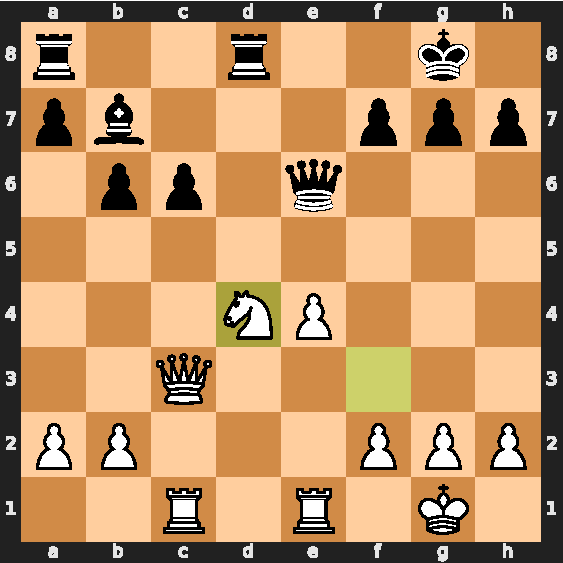
\includegraphics[width=\boardwidth]{diagrams/board-5453c1f1de42}}}

\Move{\href{https://lichess.org/analysis/pgn/d4_d5_Nf3_Nf6_c4_e6_Nc3_Nbd7_Bg5_Be7_e3_O-O_Rc1_c6_Qc2_dxc4_Bxc4_Nd5_Bxe7_Qxe7_O-O_Nxc3_Qxc3_b6_e4_Bb7_Rfe1_Rfd8_d5_Nc5_dxe6_Nxe6_Bxe6_Qxe6_Nd4_Qe5}{18...\figQ e5!}}

Of course, if \href{https://lichess.org/analysis/pgn/d4_d5_Nf3_Nf6_c4_e6_Nc3_Nbd7_Bg5_Be7_e3_O-O_Rc1_c6_Qc2_dxc4_Bxc4_Nd5_Bxe7_Qxe7_O-O_Nxc3_Qxc3_b6_e4_Bb7_Rfe1_Rfd8_d5_Nc5_dxe6_Nxe6_Bxe6_Qxe6_Nd4_Qxa2}{18...\figQ xa2} \href{https://lichess.org/analysis/pgn/d4_d5_Nf3_Nf6_c4_e6_Nc3_Nbd7_Bg5_Be7_e3_O-O_Rc1_c6_Qc2_dxc4_Bxc4_Nd5_Bxe7_Qxe7_O-O_Nxc3_Qxc3_b6_e4_Bb7_Rfe1_Rfd8_d5_Nc5_dxe6_Nxe6_Bxe6_Qxe6_Nd4_Qxa2_Ra1}{19.\figR a1} would win the Queen. The text move is probably the only satisfactory move in the position. The obvious move would have been \href{https://lichess.org/analysis/pgn/d4_d5_Nf3_Nf6_c4_e6_Nc3_Nbd7_Bg5_Be7_e3_O-O_Rc1_c6_Qc2_dxc4_Bxc4_Nd5_Bxe7_Qxe7_O-O_Nxc3_Qxc3_b6_e4_Bb7_Rfe1_Rfd8_d5_Nc5_dxe6_Nxe6_Bxe6_Qxe6_Nd4_Qd7}{18...\figQ d7} to defend the c-pawn, and then would have come \href{https://lichess.org/analysis/pgn/d4_d5_Nf3_Nf6_c4_e6_Nc3_Nbd7_Bg5_Be7_e3_O-O_Rc1_c6_Qc2_dxc4_Bxc4_Nd5_Bxe7_Qxe7_O-O_Nxc3_Qxc3_b6_e4_Bb7_Rfe1_Rfd8_d5_Nc5_dxe6_Nxe6_Bxe6_Qxe6_Nd4_Qd7_Nf5}{19.\figN f5} \href{https://lichess.org/analysis/pgn/d4_d5_Nf3_Nf6_c4_e6_Nc3_Nbd7_Bg5_Be7_e3_O-O_Rc1_c6_Qc2_dxc4_Bxc4_Nd5_Bxe7_Qxe7_O-O_Nxc3_Qxc3_b6_e4_Bb7_Rfe1_Rfd8_d5_Nc5_dxe6_Nxe6_Bxe6_Qxe6_Nd4_Qd7_Nf5_f6}{f6} \href{https://lichess.org/analysis/pgn/d4_d5_Nf3_Nf6_c4_e6_Nc3_Nbd7_Bg5_Be7_e3_O-O_Rc1_c6_Qc2_dxc4_Bxc4_Nd5_Bxe7_Qxe7_O-O_Nxc3_Qxc3_b6_e4_Bb7_Rfe1_Rfd8_d5_Nc5_dxe6_Nxe6_Bxe6_Qxe6_Nd4_Qd7_Nf5_f6_Qg3}{20.\figQ g3} (threatening \figR ad1), \href{https://lichess.org/analysis/pgn/d4_d5_Nf3_Nf6_c4_e6_Nc3_Nbd7_Bg5_Be7_e3_O-O_Rc1_c6_Qc2_dxc4_Bxc4_Nd5_Bxe7_Qxe7_O-O_Nxc3_Qxc3_b6_e4_Bb7_Rfe1_Rfd8_d5_Nc5_dxe6_Nxe6_Bxe6_Qxe6_Nd4_Qd7_Nf5_f6_Qg3_Kh8}{20...\figK h8} \href{https://lichess.org/analysis/pgn/d4_d5_Nf3_Nf6_c4_e6_Nc3_Nbd7_Bg5_Be7_e3_O-O_Rc1_c6_Qc2_dxc4_Bxc4_Nd5_Bxe7_Qxe7_O-O_Nxc3_Qxc3_b6_e4_Bb7_Rfe1_Rfd8_d5_Nc5_dxe6_Nxe6_Bxe6_Qxe6_Nd4_Qd7_Nf5_f6_Qg3_Kh8_Rcd1}{21.\figR cd1} \href{https://lichess.org/analysis/pgn/d4_d5_Nf3_Nf6_c4_e6_Nc3_Nbd7_Bg5_Be7_e3_O-O_Rc1_c6_Qc2_dxc4_Bxc4_Nd5_Bxe7_Qxe7_O-O_Nxc3_Qxc3_b6_e4_Bb7_Rfe1_Rfd8_d5_Nc5_dxe6_Nxe6_Bxe6_Qxe6_Nd4_Qd7_Nf5_f6_Qg3_Kh8_Rcd1_Qf7}{\figQ f7} \href{https://lichess.org/analysis/pgn/d4_d5_Nf3_Nf6_c4_e6_Nc3_Nbd7_Bg5_Be7_e3_O-O_Rc1_c6_Qc2_dxc4_Bxc4_Nd5_Bxe7_Qxe7_O-O_Nxc3_Qxc3_b6_e4_Bb7_Rfe1_Rfd8_d5_Nc5_dxe6_Nxe6_Bxe6_Qxe6_Nd4_Qd7_Nf5_f6_Qg3_Kh8_Rcd1_Qf7_h4}{22.h4}, with a tremendous advantage in position. The text move, on the other hand, assures Black an even game at the very least, as will soon be seen.

\Move{\href{https://lichess.org/analysis/pgn/d4_d5_Nf3_Nf6_c4_e6_Nc3_Nbd7_Bg5_Be7_e3_O-O_Rc1_c6_Qc2_dxc4_Bxc4_Nd5_Bxe7_Qxe7_O-O_Nxc3_Qxc3_b6_e4_Bb7_Rfe1_Rfd8_d5_Nc5_dxe6_Nxe6_Bxe6_Qxe6_Nd4_Qe5_Nxc6}{19.\figN xc6} \href{https://lichess.org/analysis/pgn/d4_d5_Nf3_Nf6_c4_e6_Nc3_Nbd7_Bg5_Be7_e3_O-O_Rc1_c6_Qc2_dxc4_Bxc4_Nd5_Bxe7_Qxe7_O-O_Nxc3_Qxc3_b6_e4_Bb7_Rfe1_Rfd8_d5_Nc5_dxe6_Nxe6_Bxe6_Qxe6_Nd4_Qe5_Nxc6_Qxc3}{\figQ xc3} \href{https://lichess.org/analysis/pgn/d4_d5_Nf3_Nf6_c4_e6_Nc3_Nbd7_Bg5_Be7_e3_O-O_Rc1_c6_Qc2_dxc4_Bxc4_Nd5_Bxe7_Qxe7_O-O_Nxc3_Qxc3_b6_e4_Bb7_Rfe1_Rfd8_d5_Nc5_dxe6_Nxe6_Bxe6_Qxe6_Nd4_Qe5_Nxc6_Qxc3_Rxc3}{20.\figR xc3} \href{https://lichess.org/analysis/pgn/d4_d5_Nf3_Nf6_c4_e6_Nc3_Nbd7_Bg5_Be7_e3_O-O_Rc1_c6_Qc2_dxc4_Bxc4_Nd5_Bxe7_Qxe7_O-O_Nxc3_Qxc3_b6_e4_Bb7_Rfe1_Rfd8_d5_Nc5_dxe6_Nxe6_Bxe6_Qxe6_Nd4_Qe5_Nxc6_Qxc3_Rxc3_Rd2}{\figR d2} \href{https://lichess.org/analysis/pgn/d4_d5_Nf3_Nf6_c4_e6_Nc3_Nbd7_Bg5_Be7_e3_O-O_Rc1_c6_Qc2_dxc4_Bxc4_Nd5_Bxe7_Qxe7_O-O_Nxc3_Qxc3_b6_e4_Bb7_Rfe1_Rfd8_d5_Nc5_dxe6_Nxe6_Bxe6_Qxe6_Nd4_Qe5_Nxc6_Qxc3_Rxc3_Rd2_Rb1}{21.\figR b1}}

A very serious error of judgment. White is under the impression that he has the better game, because he is a Pawn ahead, but that is not so. The powerful position of the Black Rook at d2 fully compensates Black for the Pawn minus. Besides, the Bishop is better with Rooks than the Knight (see pages 48--56, where the relative values of the Knight and Bishop are compared), and, as already stated, with Pawns on both sides of the board the Bishop is superior because of its long range. Incidentally, this ending will demonstrate the great power of the Bishop. White's best chance was to take a draw at once, thus. \href{https://lichess.org/analysis/pgn/d4_d5_Nf3_Nf6_c4_e6_Nc3_Nbd7_Bg5_Be7_e3_O-O_Rc1_c6_Qc2_dxc4_Bxc4_Nd5_Bxe7_Qxe7_O-O_Nxc3_Qxc3_b6_e4_Bb7_Rfe1_Rfd8_d5_Nc5_dxe6_Nxe6_Bxe6_Qxe6_Nd4_Qe5_Nxc6_Qxc3_Rxc3_Rd2_Ne7}{21.\figN e7+} \href{https://lichess.org/analysis/pgn/d4_d5_Nf3_Nf6_c4_e6_Nc3_Nbd7_Bg5_Be7_e3_O-O_Rc1_c6_Qc2_dxc4_Bxc4_Nd5_Bxe7_Qxe7_O-O_Nxc3_Qxc3_b6_e4_Bb7_Rfe1_Rfd8_d5_Nc5_dxe6_Nxe6_Bxe6_Qxe6_Nd4_Qe5_Nxc6_Qxc3_Rxc3_Rd2_Ne7_Kf8}{\figK f8} \href{https://lichess.org/analysis/pgn/d4_d5_Nf3_Nf6_c4_e6_Nc3_Nbd7_Bg5_Be7_e3_O-O_Rc1_c6_Qc2_dxc4_Bxc4_Nd5_Bxe7_Qxe7_O-O_Nxc3_Qxc3_b6_e4_Bb7_Rfe1_Rfd8_d5_Nc5_dxe6_Nxe6_Bxe6_Qxe6_Nd4_Qe5_Nxc6_Qxc3_Rxc3_Rd2_Ne7_Kf8_Rc7}{22.\figR c7} \href{https://lichess.org/analysis/pgn/d4_d5_Nf3_Nf6_c4_e6_Nc3_Nbd7_Bg5_Be7_e3_O-O_Rc1_c6_Qc2_dxc4_Bxc4_Nd5_Bxe7_Qxe7_O-O_Nxc3_Qxc3_b6_e4_Bb7_Rfe1_Rfd8_d5_Nc5_dxe6_Nxe6_Bxe6_Qxe6_Nd4_Qe5_Nxc6_Qxc3_Rxc3_Rd2_Ne7_Kf8_Rc7_Re8}{22...\figR e8} (not \figB xe4; because f3 would give White the best of it); \href{https://lichess.org/analysis/pgn/d4_d5_Nf3_Nf6_c4_e6_Nc3_Nbd7_Bg5_Be7_e3_O-O_Rc1_c6_Qc2_dxc4_Bxc4_Nd5_Bxe7_Qxe7_O-O_Nxc3_Qxc3_b6_e4_Bb7_Rfe1_Rfd8_d5_Nc5_dxe6_Nxe6_Bxe6_Qxe6_Nd4_Qe5_Nxc6_Qxc3_Rxc3_Rd2_Ne7_Kf8_Rc7_Re8_Rxb7}{23.\figR xb7} (best; not \figN g6+, because of ...fxg6; followed by \figR xe4), \href{https://lichess.org/analysis/pgn/d4_d5_Nf3_Nf6_c4_e6_Nc3_Nbd7_Bg5_Be7_e3_O-O_Rc1_c6_Qc2_dxc4_Bxc4_Nd5_Bxe7_Qxe7_O-O_Nxc3_Qxc3_b6_e4_Bb7_Rfe1_Rfd8_d5_Nc5_dxe6_Nxe6_Bxe6_Qxe6_Nd4_Qe5_Nxc6_Qxc3_Rxc3_Rd2_Ne7_Kf8_Rc7_Re8_Rxb7_Rxe7}{23...\figR xe7} \href{https://lichess.org/analysis/pgn/d4_d5_Nf3_Nf6_c4_e6_Nc3_Nbd7_Bg5_Be7_e3_O-O_Rc1_c6_Qc2_dxc4_Bxc4_Nd5_Bxe7_Qxe7_O-O_Nxc3_Qxc3_b6_e4_Bb7_Rfe1_Rfd8_d5_Nc5_dxe6_Nxe6_Bxe6_Qxe6_Nd4_Qe5_Nxc6_Qxc3_Rxc3_Rd2_Ne7_Kf8_Rc7_Re8_Rxb7_Rxe7_Rb8}{24.\figR b8+} \href{https://lichess.org/analysis/pgn/d4_d5_Nf3_Nf6_c4_e6_Nc3_Nbd7_Bg5_Be7_e3_O-O_Rc1_c6_Qc2_dxc4_Bxc4_Nd5_Bxe7_Qxe7_O-O_Nxc3_Qxc3_b6_e4_Bb7_Rfe1_Rfd8_d5_Nc5_dxe6_Nxe6_Bxe6_Qxe6_Nd4_Qe5_Nxc6_Qxc3_Rxc3_Rd2_Ne7_Kf8_Rc7_Re8_Rxb7_Rxe7_Rb8_Re8}{\figR e8} \href{https://lichess.org/analysis/pgn/d4_d5_Nf3_Nf6_c4_e6_Nc3_Nbd7_Bg5_Be7_e3_O-O_Rc1_c6_Qc2_dxc4_Bxc4_Nd5_Bxe7_Qxe7_O-O_Nxc3_Qxc3_b6_e4_Bb7_Rfe1_Rfd8_d5_Nc5_dxe6_Nxe6_Bxe6_Qxe6_Nd4_Qe5_Nxc6_Qxc3_Rxc3_Rd2_Ne7_Kf8_Rc7_Re8_Rxb7_Rxe7_Rb8_Re8_Rxe8}{25.\figR xe8+} \href{https://lichess.org/analysis/pgn/d4_d5_Nf3_Nf6_c4_e6_Nc3_Nbd7_Bg5_Be7_e3_O-O_Rc1_c6_Qc2_dxc4_Bxc4_Nd5_Bxe7_Qxe7_O-O_Nxc3_Qxc3_b6_e4_Bb7_Rfe1_Rfd8_d5_Nc5_dxe6_Nxe6_Bxe6_Qxe6_Nd4_Qe5_Nxc6_Qxc3_Rxc3_Rd2_Ne7_Kf8_Rc7_Re8_Rxb7_Rxe7_Rb8_Re8_Rxe8_Kxe8}{\figK xe8}, and with proper play White will draw.

It is curious that, although a Pawn ahead, White is the one who is always in danger. It is only now, after seeing this analysis, that the value of Black's 18th move \href{https://lichess.org/analysis/pgn/d4_d5_Nf3_Nf6_c4_e6_Nc3_Nbd7_Bg5_Be7_e3_O-O_Rc1_c6_Qc2_dxc4_Bxc4_Nd5_Bxe7_Qxe7_O-O_Nxc3_Qxc3_b6_e4_Bb7_Rfe1_Rfd8_d5_Nc5_dxe6_Nxe6_Bxe6_Qxe6_Nd4_Qe5}{18...\figQ e5} can be fully appreciated.

\Move{\href{https://lichess.org/analysis/pgn/d4_d5_Nf3_Nf6_c4_e6_Nc3_Nbd7_Bg5_Be7_e3_O-O_Rc1_c6_Qc2_dxc4_Bxc4_Nd5_Bxe7_Qxe7_O-O_Nxc3_Qxc3_b6_e4_Bb7_Rfe1_Rfd8_d5_Nc5_dxe6_Nxe6_Bxe6_Qxe6_Nd4_Qe5_Nxc6_Qxc3_Rxc3_Rd2_Rb1_Re8}{21...\figR e8}}

With this powerful move Black begins, against White's centre, an assault which will soon be shifted against the King itself. White is afraid to play \href{https://lichess.org/analysis/pgn/d4_d5_Nf3_Nf6_c4_e6_Nc3_Nbd7_Bg5_Be7_e3_O-O_Rc1_c6_Qc2_dxc4_Bxc4_Nd5_Bxe7_Qxe7_O-O_Nxc3_Qxc3_b6_e4_Bb7_Rfe1_Rfd8_d5_Nc5_dxe6_Nxe6_Bxe6_Qxe6_Nd4_Qe5_Nxc6_Qxc3_Rxc3_Rd2_Rb1_Re8_f3}{22.f3} because of ...f5.

\Move{\href{https://lichess.org/analysis/pgn/d4_d5_Nf3_Nf6_c4_e6_Nc3_Nbd7_Bg5_Be7_e3_O-O_Rc1_c6_Qc2_dxc4_Bxc4_Nd5_Bxe7_Qxe7_O-O_Nxc3_Qxc3_b6_e4_Bb7_Rfe1_Rfd8_d5_Nc5_dxe6_Nxe6_Bxe6_Qxe6_Nd4_Qe5_Nxc6_Qxc3_Rxc3_Rd2_Rb1_Re8_e5}{22.e5} \href{https://lichess.org/analysis/pgn/d4_d5_Nf3_Nf6_c4_e6_Nc3_Nbd7_Bg5_Be7_e3_O-O_Rc1_c6_Qc2_dxc4_Bxc4_Nd5_Bxe7_Qxe7_O-O_Nxc3_Qxc3_b6_e4_Bb7_Rfe1_Rfd8_d5_Nc5_dxe6_Nxe6_Bxe6_Qxe6_Nd4_Qe5_Nxc6_Qxc3_Rxc3_Rd2_Rb1_Re8_e5_g5}{g5}}

To prevent f4. The White Knight is practically pinned, because he does not dare move on account of \figR xe5.

\ChessDiagram{\href{https://lichess.org/analysis/pgn/d4_d5_Nf3_Nf6_c4_e6_Nc3_Nbd7_Bg5_Be7_e3_O-O_Rc1_c6_Qc2_dxc4_Bxc4_Nd5_Bxe7_Qxe7_O-O_Nxc3_Qxc3_b6_e4_Bb7_Rfe1_Rfd8_d5_Nc5_dxe6_Nxe6_Bxe6_Qxe6_Nd4_Qe5_Nxc6_Qxc3_Rxc3_Rd2_Rb1_Re8_e5_g5}{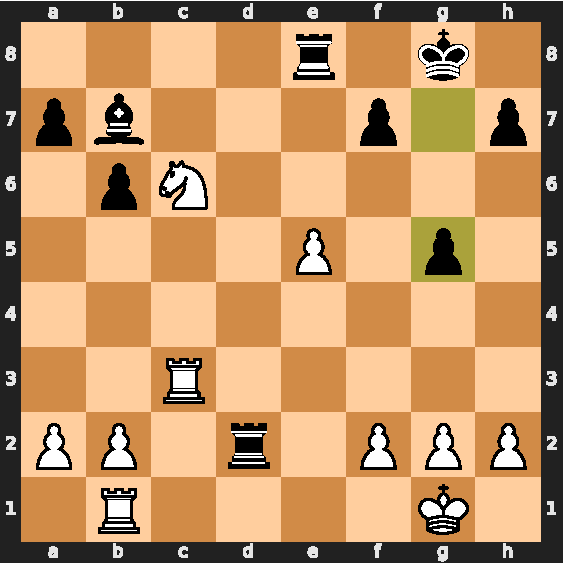
\includegraphics[width=\boardwidth]{diagrams/board-5c296999d321}}}

\Move{\href{https://lichess.org/analysis/pgn/d4_d5_Nf3_Nf6_c4_e6_Nc3_Nbd7_Bg5_Be7_e3_O-O_Rc1_c6_Qc2_dxc4_Bxc4_Nd5_Bxe7_Qxe7_O-O_Nxc3_Qxc3_b6_e4_Bb7_Rfe1_Rfd8_d5_Nc5_dxe6_Nxe6_Bxe6_Qxe6_Nd4_Qe5_Nxc6_Qxc3_Rxc3_Rd2_Rb1_Re8_e5_g5_h4}{23.h4}}

This is a sequel to the previous move. White expects to disrupt Black's Pawns, and thus make them weak.

\Move{\href{https://lichess.org/analysis/pgn/d4_d5_Nf3_Nf6_c4_e6_Nc3_Nbd7_Bg5_Be7_e3_O-O_Rc1_c6_Qc2_dxc4_Bxc4_Nd5_Bxe7_Qxe7_O-O_Nxc3_Qxc3_b6_e4_Bb7_Rfe1_Rfd8_d5_Nc5_dxe6_Nxe6_Bxe6_Qxe6_Nd4_Qe5_Nxc6_Qxc3_Rxc3_Rd2_Rb1_Re8_e5_g5_h4_gxh4}{23...gxh4}}

Though doubled and isolated this Pawn exercises enormous pressure. Black now threatens \figR e6; to be followed by \figR g6 and ...h3 and h2 at the proper time.

\Move{\href{https://lichess.org/analysis/pgn/d4_d5_Nf3_Nf6_c4_e6_Nc3_Nbd7_Bg5_Be7_e3_O-O_Rc1_c6_Qc2_dxc4_Bxc4_Nd5_Bxe7_Qxe7_O-O_Nxc3_Qxc3_b6_e4_Bb7_Rfe1_Rfd8_d5_Nc5_dxe6_Nxe6_Bxe6_Qxe6_Nd4_Qe5_Nxc6_Qxc3_Rxc3_Rd2_Rb1_Re8_e5_g5_h4_gxh4_Re1}{24.\figR e1}}

White cannot stand the slow death any longer. He sees danger everywhere, and wants to avert it by giving up his Queen's side Pawns, expecting to regain his fortunes later on by taking the initiative on the King's side.

\Move{\href{https://lichess.org/analysis/pgn/d4_d5_Nf3_Nf6_c4_e6_Nc3_Nbd7_Bg5_Be7_e3_O-O_Rc1_c6_Qc2_dxc4_Bxc4_Nd5_Bxe7_Qxe7_O-O_Nxc3_Qxc3_b6_e4_Bb7_Rfe1_Rfd8_d5_Nc5_dxe6_Nxe6_Bxe6_Qxe6_Nd4_Qe5_Nxc6_Qxc3_Rxc3_Rd2_Rb1_Re8_e5_g5_h4_gxh4_Re1_Re6}{24...\figR e6!}}

Much better than taking Pawns. This forces White to defend the Knight with the Rook at e1, because of the threat \figR g6.

\Move{\href{https://lichess.org/analysis/pgn/d4_d5_Nf3_Nf6_c4_e6_Nc3_Nbd7_Bg5_Be7_e3_O-O_Rc1_c6_Qc2_dxc4_Bxc4_Nd5_Bxe7_Qxe7_O-O_Nxc3_Qxc3_b6_e4_Bb7_Rfe1_Rfd8_d5_Nc5_dxe6_Nxe6_Bxe6_Qxe6_Nd4_Qe5_Nxc6_Qxc3_Rxc3_Rd2_Rb1_Re8_e5_g5_h4_gxh4_Re1_Re6_Rec1}{25.\figR ec1} \href{https://lichess.org/analysis/pgn/d4_d5_Nf3_Nf6_c4_e6_Nc3_Nbd7_Bg5_Be7_e3_O-O_Rc1_c6_Qc2_dxc4_Bxc4_Nd5_Bxe7_Qxe7_O-O_Nxc3_Qxc3_b6_e4_Bb7_Rfe1_Rfd8_d5_Nc5_dxe6_Nxe6_Bxe6_Qxe6_Nd4_Qe5_Nxc6_Qxc3_Rxc3_Rd2_Rb1_Re8_e5_g5_h4_gxh4_Re1_Re6_Rec1_Kg7}{\figK g7}}

Preparatory to \figR g6. The game is going to be decided on the King's side, and it is the isolated double Pawn that will supply the finishing touch.

\Move{\href{https://lichess.org/analysis/pgn/d4_d5_Nf3_Nf6_c4_e6_Nc3_Nbd7_Bg5_Be7_e3_O-O_Rc1_c6_Qc2_dxc4_Bxc4_Nd5_Bxe7_Qxe7_O-O_Nxc3_Qxc3_b6_e4_Bb7_Rfe1_Rfd8_d5_Nc5_dxe6_Nxe6_Bxe6_Qxe6_Nd4_Qe5_Nxc6_Qxc3_Rxc3_Rd2_Rb1_Re8_e5_g5_h4_gxh4_Re1_Re6_Rec1_Kg7_b4}{26.b4} \href{https://lichess.org/analysis/pgn/d4_d5_Nf3_Nf6_c4_e6_Nc3_Nbd7_Bg5_Be7_e3_O-O_Rc1_c6_Qc2_dxc4_Bxc4_Nd5_Bxe7_Qxe7_O-O_Nxc3_Qxc3_b6_e4_Bb7_Rfe1_Rfd8_d5_Nc5_dxe6_Nxe6_Bxe6_Qxe6_Nd4_Qe5_Nxc6_Qxc3_Rxc3_Rd2_Rb1_Re8_e5_g5_h4_gxh4_Re1_Re6_Rec1_Kg7_b4_b5}{b5}}

To prevent b5, defending the Knight and liberating the Rooks.

\Move{\href{https://lichess.org/analysis/pgn/d4_d5_Nf3_Nf6_c4_e6_Nc3_Nbd7_Bg5_Be7_e3_O-O_Rc1_c6_Qc2_dxc4_Bxc4_Nd5_Bxe7_Qxe7_O-O_Nxc3_Qxc3_b6_e4_Bb7_Rfe1_Rfd8_d5_Nc5_dxe6_Nxe6_Bxe6_Qxe6_Nd4_Qe5_Nxc6_Qxc3_Rxc3_Rd2_Rb1_Re8_e5_g5_h4_gxh4_Re1_Re6_Rec1_Kg7_b4_b5_a3}{27.a3} \href{https://lichess.org/analysis/pgn/d4_d5_Nf3_Nf6_c4_e6_Nc3_Nbd7_Bg5_Be7_e3_O-O_Rc1_c6_Qc2_dxc4_Bxc4_Nd5_Bxe7_Qxe7_O-O_Nxc3_Qxc3_b6_e4_Bb7_Rfe1_Rfd8_d5_Nc5_dxe6_Nxe6_Bxe6_Qxe6_Nd4_Qe5_Nxc6_Qxc3_Rxc3_Rd2_Rb1_Re8_e5_g5_h4_gxh4_Re1_Re6_Rec1_Kg7_b4_b5_a3_Rg6}{\figR g6} \href{https://lichess.org/analysis/pgn/d4_d5_Nf3_Nf6_c4_e6_Nc3_Nbd7_Bg5_Be7_e3_O-O_Rc1_c6_Qc2_dxc4_Bxc4_Nd5_Bxe7_Qxe7_O-O_Nxc3_Qxc3_b6_e4_Bb7_Rfe1_Rfd8_d5_Nc5_dxe6_Nxe6_Bxe6_Qxe6_Nd4_Qe5_Nxc6_Qxc3_Rxc3_Rd2_Rb1_Re8_e5_g5_h4_gxh4_Re1_Re6_Rec1_Kg7_b4_b5_a3_Rg6_Kf1}{28.\figK f1} \href{https://lichess.org/analysis/pgn/d4_d5_Nf3_Nf6_c4_e6_Nc3_Nbd7_Bg5_Be7_e3_O-O_Rc1_c6_Qc2_dxc4_Bxc4_Nd5_Bxe7_Qxe7_O-O_Nxc3_Qxc3_b6_e4_Bb7_Rfe1_Rfd8_d5_Nc5_dxe6_Nxe6_Bxe6_Qxe6_Nd4_Qe5_Nxc6_Qxc3_Rxc3_Rd2_Rb1_Re8_e5_g5_h4_gxh4_Re1_Re6_Rec1_Kg7_b4_b5_a3_Rg6_Kf1_Ra2}{\figR a2}}

\ChessDiagram{\href{https://lichess.org/analysis/pgn/d4_d5_Nf3_Nf6_c4_e6_Nc3_Nbd7_Bg5_Be7_e3_O-O_Rc1_c6_Qc2_dxc4_Bxc4_Nd5_Bxe7_Qxe7_O-O_Nxc3_Qxc3_b6_e4_Bb7_Rfe1_Rfd8_d5_Nc5_dxe6_Nxe6_Bxe6_Qxe6_Nd4_Qe5_Nxc6_Qxc3_Rxc3_Rd2_Rb1_Re8_e5_g5_h4_gxh4_Re1_Re6_Rec1_Kg7_b4_b5_a3_Rg6_Kf1_Ra2}{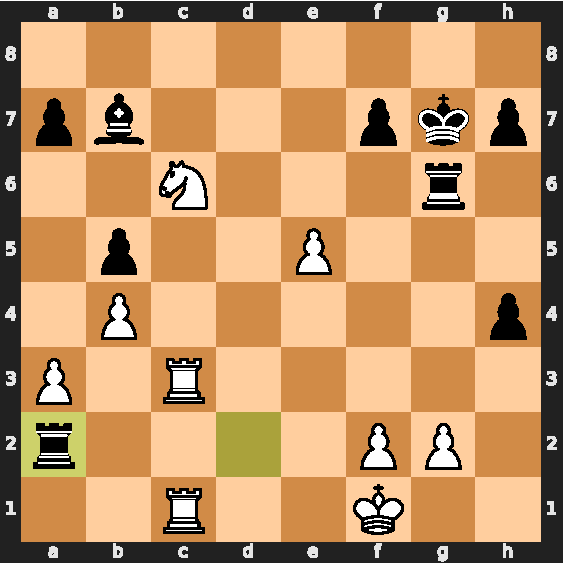
\includegraphics[width=\boardwidth]{diagrams/board-aea232c967ec}}}

Notice the remarkable position of the pieces. White cannot move anything without incurring some loss. His best chance would have been to play \href{https://lichess.org/analysis/pgn/d4_d5_Nf3_Nf6_c4_e6_Nc3_Nbd7_Bg5_Be7_e3_O-O_Rc1_c6_Qc2_dxc4_Bxc4_Nd5_Bxe7_Qxe7_O-O_Nxc3_Qxc3_b6_e4_Bb7_Rfe1_Rfd8_d5_Nc5_dxe6_Nxe6_Bxe6_Qxe6_Nd4_Qe5_Nxc6_Qxc3_Rxc3_Rd2_Rb1_Re8_e5_g5_h4_gxh4_Re1_Re6_Rec1_Kg7_b4_b5_a3_Rg6_Kf1_Ra2_e6}{29.e6}, but that would only have prolonged the game, which is lost in any case.

\Move{\href{https://lichess.org/analysis/pgn/d4_d5_Nf3_Nf6_c4_e6_Nc3_Nbd7_Bg5_Be7_e3_O-O_Rc1_c6_Qc2_dxc4_Bxc4_Nd5_Bxe7_Qxe7_O-O_Nxc3_Qxc3_b6_e4_Bb7_Rfe1_Rfd8_d5_Nc5_dxe6_Nxe6_Bxe6_Qxe6_Nd4_Qe5_Nxc6_Qxc3_Rxc3_Rd2_Rb1_Re8_e5_g5_h4_gxh4_Re1_Re6_Rec1_Kg7_b4_b5_a3_Rg6_Kf1_Ra2_Kg1}{29.\figK g1} \href{https://lichess.org/analysis/pgn/d4_d5_Nf3_Nf6_c4_e6_Nc3_Nbd7_Bg5_Be7_e3_O-O_Rc1_c6_Qc2_dxc4_Bxc4_Nd5_Bxe7_Qxe7_O-O_Nxc3_Qxc3_b6_e4_Bb7_Rfe1_Rfd8_d5_Nc5_dxe6_Nxe6_Bxe6_Qxe6_Nd4_Qe5_Nxc6_Qxc3_Rxc3_Rd2_Rb1_Re8_e5_g5_h4_gxh4_Re1_Re6_Rec1_Kg7_b4_b5_a3_Rg6_Kf1_Ra2_Kg1_h3}{h3} \href{https://lichess.org/analysis/pgn/d4_d5_Nf3_Nf6_c4_e6_Nc3_Nbd7_Bg5_Be7_e3_O-O_Rc1_c6_Qc2_dxc4_Bxc4_Nd5_Bxe7_Qxe7_O-O_Nxc3_Qxc3_b6_e4_Bb7_Rfe1_Rfd8_d5_Nc5_dxe6_Nxe6_Bxe6_Qxe6_Nd4_Qe5_Nxc6_Qxc3_Rxc3_Rd2_Rb1_Re8_e5_g5_h4_gxh4_Re1_Re6_Rec1_Kg7_b4_b5_a3_Rg6_Kf1_Ra2_Kg1_h3_g3}{30.g3} \href{https://lichess.org/analysis/pgn/d4_d5_Nf3_Nf6_c4_e6_Nc3_Nbd7_Bg5_Be7_e3_O-O_Rc1_c6_Qc2_dxc4_Bxc4_Nd5_Bxe7_Qxe7_O-O_Nxc3_Qxc3_b6_e4_Bb7_Rfe1_Rfd8_d5_Nc5_dxe6_Nxe6_Bxe6_Qxe6_Nd4_Qe5_Nxc6_Qxc3_Rxc3_Rd2_Rb1_Re8_e5_g5_h4_gxh4_Re1_Re6_Rec1_Kg7_b4_b5_a3_Rg6_Kf1_Ra2_Kg1_h3_g3_a6}{a6}}

Again forcing White to move and to lose something thereby, as all his pieces are tied up.

\ChessDiagram{\href{https://lichess.org/analysis/pgn/d4_d5_Nf3_Nf6_c4_e6_Nc3_Nbd7_Bg5_Be7_e3_O-O_Rc1_c6_Qc2_dxc4_Bxc4_Nd5_Bxe7_Qxe7_O-O_Nxc3_Qxc3_b6_e4_Bb7_Rfe1_Rfd8_d5_Nc5_dxe6_Nxe6_Bxe6_Qxe6_Nd4_Qe5_Nxc6_Qxc3_Rxc3_Rd2_Rb1_Re8_e5_g5_h4_gxh4_Re1_Re6_Rec1_Kg7_b4_b5_a3_Rg6_Kf1_Ra2_Kg1_h3_g3_a6}{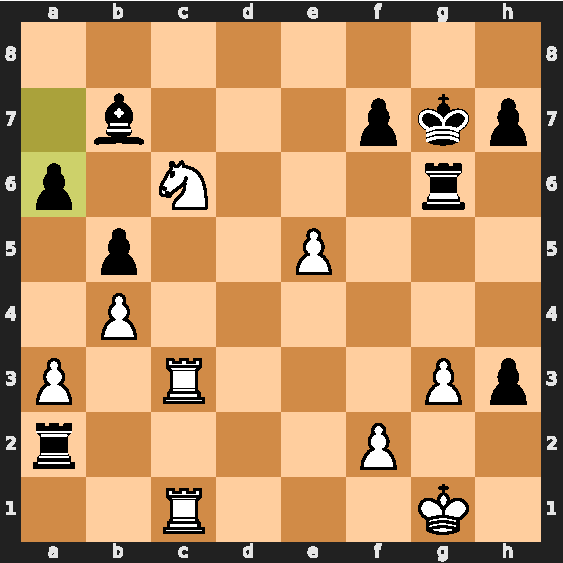
\includegraphics[width=\boardwidth]{diagrams/board-b1a87dd86145}}}

\Move{\href{https://lichess.org/analysis/pgn/d4_d5_Nf3_Nf6_c4_e6_Nc3_Nbd7_Bg5_Be7_e3_O-O_Rc1_c6_Qc2_dxc4_Bxc4_Nd5_Bxe7_Qxe7_O-O_Nxc3_Qxc3_b6_e4_Bb7_Rfe1_Rfd8_d5_Nc5_dxe6_Nxe6_Bxe6_Qxe6_Nd4_Qe5_Nxc6_Qxc3_Rxc3_Rd2_Rb1_Re8_e5_g5_h4_gxh4_Re1_Re6_Rec1_Kg7_b4_b5_a3_Rg6_Kf1_Ra2_Kg1_h3_g3_a6_e6}{31.e6} \href{https://lichess.org/analysis/pgn/d4_d5_Nf3_Nf6_c4_e6_Nc3_Nbd7_Bg5_Be7_e3_O-O_Rc1_c6_Qc2_dxc4_Bxc4_Nd5_Bxe7_Qxe7_O-O_Nxc3_Qxc3_b6_e4_Bb7_Rfe1_Rfd8_d5_Nc5_dxe6_Nxe6_Bxe6_Qxe6_Nd4_Qe5_Nxc6_Qxc3_Rxc3_Rd2_Rb1_Re8_e5_g5_h4_gxh4_Re1_Re6_Rec1_Kg7_b4_b5_a3_Rg6_Kf1_Ra2_Kg1_h3_g3_a6_e6_Rxe6}{\figR xe6}}

Not even now can White move the Knight because of ...h2+; \figK xh2, \figR h6+; \figK g1, \figR h1 mate.

\Move{\href{https://lichess.org/analysis/pgn/d4_d5_Nf3_Nf6_c4_e6_Nc3_Nbd7_Bg5_Be7_e3_O-O_Rc1_c6_Qc2_dxc4_Bxc4_Nd5_Bxe7_Qxe7_O-O_Nxc3_Qxc3_b6_e4_Bb7_Rfe1_Rfd8_d5_Nc5_dxe6_Nxe6_Bxe6_Qxe6_Nd4_Qe5_Nxc6_Qxc3_Rxc3_Rd2_Rb1_Re8_e5_g5_h4_gxh4_Re1_Re6_Rec1_Kg7_b4_b5_a3_Rg6_Kf1_Ra2_Kg1_h3_g3_a6_e6_Rxe6_g4}{32.g4} \href{https://lichess.org/analysis/pgn/d4_d5_Nf3_Nf6_c4_e6_Nc3_Nbd7_Bg5_Be7_e3_O-O_Rc1_c6_Qc2_dxc4_Bxc4_Nd5_Bxe7_Qxe7_O-O_Nxc3_Qxc3_b6_e4_Bb7_Rfe1_Rfd8_d5_Nc5_dxe6_Nxe6_Bxe6_Qxe6_Nd4_Qe5_Nxc6_Qxc3_Rxc3_Rd2_Rb1_Re8_e5_g5_h4_gxh4_Re1_Re6_Rec1_Kg7_b4_b5_a3_Rg6_Kf1_Ra2_Kg1_h3_g3_a6_e6_Rxe6_g4_Rh6}{\figR h6} \href{https://lichess.org/analysis/pgn/d4_d5_Nf3_Nf6_c4_e6_Nc3_Nbd7_Bg5_Be7_e3_O-O_Rc1_c6_Qc2_dxc4_Bxc4_Nd5_Bxe7_Qxe7_O-O_Nxc3_Qxc3_b6_e4_Bb7_Rfe1_Rfd8_d5_Nc5_dxe6_Nxe6_Bxe6_Qxe6_Nd4_Qe5_Nxc6_Qxc3_Rxc3_Rd2_Rb1_Re8_e5_g5_h4_gxh4_Re1_Re6_Rec1_Kg7_b4_b5_a3_Rg6_Kf1_Ra2_Kg1_h3_g3_a6_e6_Rxe6_g4_Rh6_f3}{33.f3}}

If \href{https://lichess.org/analysis/pgn/d4_d5_Nf3_Nf6_c4_e6_Nc3_Nbd7_Bg5_Be7_e3_O-O_Rc1_c6_Qc2_dxc4_Bxc4_Nd5_Bxe7_Qxe7_O-O_Nxc3_Qxc3_b6_e4_Bb7_Rfe1_Rfd8_d5_Nc5_dxe6_Nxe6_Bxe6_Qxe6_Nd4_Qe5_Nxc6_Qxc3_Rxc3_Rd2_Rb1_Re8_e5_g5_h4_gxh4_Re1_Re6_Rec1_Kg7_b4_b5_a3_Rg6_Kf1_Ra2_Kg1_h3_g3_a6_e6_Rxe6_g4_Rh6_g5}{33.g5} \href{https://lichess.org/analysis/pgn/d4_d5_Nf3_Nf6_c4_e6_Nc3_Nbd7_Bg5_Be7_e3_O-O_Rc1_c6_Qc2_dxc4_Bxc4_Nd5_Bxe7_Qxe7_O-O_Nxc3_Qxc3_b6_e4_Bb7_Rfe1_Rfd8_d5_Nc5_dxe6_Nxe6_Bxe6_Qxe6_Nd4_Qe5_Nxc6_Qxc3_Rxc3_Rd2_Rb1_Re8_e5_g5_h4_gxh4_Re1_Re6_Rec1_Kg7_b4_b5_a3_Rg6_Kf1_Ra2_Kg1_h3_g3_a6_e6_Rxe6_g4_Rh6_g5_h2}{h2+} \href{https://lichess.org/analysis/pgn/d4_d5_Nf3_Nf6_c4_e6_Nc3_Nbd7_Bg5_Be7_e3_O-O_Rc1_c6_Qc2_dxc4_Bxc4_Nd5_Bxe7_Qxe7_O-O_Nxc3_Qxc3_b6_e4_Bb7_Rfe1_Rfd8_d5_Nc5_dxe6_Nxe6_Bxe6_Qxe6_Nd4_Qe5_Nxc6_Qxc3_Rxc3_Rd2_Rb1_Re8_e5_g5_h4_gxh4_Re1_Re6_Rec1_Kg7_b4_b5_a3_Rg6_Kf1_Ra2_Kg1_h3_g3_a6_e6_Rxe6_g4_Rh6_g5_h2_Kh1}{34.\figK h1} \href{https://lichess.org/analysis/pgn/d4_d5_Nf3_Nf6_c4_e6_Nc3_Nbd7_Bg5_Be7_e3_O-O_Rc1_c6_Qc2_dxc4_Bxc4_Nd5_Bxe7_Qxe7_O-O_Nxc3_Qxc3_b6_e4_Bb7_Rfe1_Rfd8_d5_Nc5_dxe6_Nxe6_Bxe6_Qxe6_Nd4_Qe5_Nxc6_Qxc3_Rxc3_Rd2_Rb1_Re8_e5_g5_h4_gxh4_Re1_Re6_Rec1_Kg7_b4_b5_a3_Rg6_Kf1_Ra2_Kg1_h3_g3_a6_e6_Rxe6_g4_Rh6_g5_h2_Kh1_Rxc6}{\figR xc6} \href{https://lichess.org/analysis/pgn/d4_d5_Nf3_Nf6_c4_e6_Nc3_Nbd7_Bg5_Be7_e3_O-O_Rc1_c6_Qc2_dxc4_Bxc4_Nd5_Bxe7_Qxe7_O-O_Nxc3_Qxc3_b6_e4_Bb7_Rfe1_Rfd8_d5_Nc5_dxe6_Nxe6_Bxe6_Qxe6_Nd4_Qe5_Nxc6_Qxc3_Rxc3_Rd2_Rb1_Re8_e5_g5_h4_gxh4_Re1_Re6_Rec1_Kg7_b4_b5_a3_Rg6_Kf1_Ra2_Kg1_h3_g3_a6_e6_Rxe6_g4_Rh6_g5_h2_Kh1_Rxc6_Rxc6}{35.\figR xc6} \href{https://lichess.org/analysis/pgn/d4_d5_Nf3_Nf6_c4_e6_Nc3_Nbd7_Bg5_Be7_e3_O-O_Rc1_c6_Qc2_dxc4_Bxc4_Nd5_Bxe7_Qxe7_O-O_Nxc3_Qxc3_b6_e4_Bb7_Rfe1_Rfd8_d5_Nc5_dxe6_Nxe6_Bxe6_Qxe6_Nd4_Qe5_Nxc6_Qxc3_Rxc3_Rd2_Rb1_Re8_e5_g5_h4_gxh4_Re1_Re6_Rec1_Kg7_b4_b5_a3_Rg6_Kf1_Ra2_Kg1_h3_g3_a6_e6_Rxe6_g4_Rh6_g5_h2_Kh1_Rxc6_Rxc6_Rxf2}{\figR xf2}, winning easily.

\Move{\href{https://lichess.org/analysis/pgn/d4_d5_Nf3_Nf6_c4_e6_Nc3_Nbd7_Bg5_Be7_e3_O-O_Rc1_c6_Qc2_dxc4_Bxc4_Nd5_Bxe7_Qxe7_O-O_Nxc3_Qxc3_b6_e4_Bb7_Rfe1_Rfd8_d5_Nc5_dxe6_Nxe6_Bxe6_Qxe6_Nd4_Qe5_Nxc6_Qxc3_Rxc3_Rd2_Rb1_Re8_e5_g5_h4_gxh4_Re1_Re6_Rec1_Kg7_b4_b5_a3_Rg6_Kf1_Ra2_Kg1_h3_g3_a6_e6_Rxe6_g4_Rh6_f3_Rd6}{33...\figR d6} \href{https://lichess.org/analysis/pgn/d4_d5_Nf3_Nf6_c4_e6_Nc3_Nbd7_Bg5_Be7_e3_O-O_Rc1_c6_Qc2_dxc4_Bxc4_Nd5_Bxe7_Qxe7_O-O_Nxc3_Qxc3_b6_e4_Bb7_Rfe1_Rfd8_d5_Nc5_dxe6_Nxe6_Bxe6_Qxe6_Nd4_Qe5_Nxc6_Qxc3_Rxc3_Rd2_Rb1_Re8_e5_g5_h4_gxh4_Re1_Re6_Rec1_Kg7_b4_b5_a3_Rg6_Kf1_Ra2_Kg1_h3_g3_a6_e6_Rxe6_g4_Rh6_f3_Rd6_Ne7}{34.\figN e7} \href{https://lichess.org/analysis/pgn/d4_d5_Nf3_Nf6_c4_e6_Nc3_Nbd7_Bg5_Be7_e3_O-O_Rc1_c6_Qc2_dxc4_Bxc4_Nd5_Bxe7_Qxe7_O-O_Nxc3_Qxc3_b6_e4_Bb7_Rfe1_Rfd8_d5_Nc5_dxe6_Nxe6_Bxe6_Qxe6_Nd4_Qe5_Nxc6_Qxc3_Rxc3_Rd2_Rb1_Re8_e5_g5_h4_gxh4_Re1_Re6_Rec1_Kg7_b4_b5_a3_Rg6_Kf1_Ra2_Kg1_h3_g3_a6_e6_Rxe6_g4_Rh6_f3_Rd6_Ne7_Rdd2}{\figR dd2} \href{https://lichess.org/analysis/pgn/d4_d5_Nf3_Nf6_c4_e6_Nc3_Nbd7_Bg5_Be7_e3_O-O_Rc1_c6_Qc2_dxc4_Bxc4_Nd5_Bxe7_Qxe7_O-O_Nxc3_Qxc3_b6_e4_Bb7_Rfe1_Rfd8_d5_Nc5_dxe6_Nxe6_Bxe6_Qxe6_Nd4_Qe5_Nxc6_Qxc3_Rxc3_Rd2_Rb1_Re8_e5_g5_h4_gxh4_Re1_Re6_Rec1_Kg7_b4_b5_a3_Rg6_Kf1_Ra2_Kg1_h3_g3_a6_e6_Rxe6_g4_Rh6_f3_Rd6_Ne7_Rdd2_Nf5}{35.\figN f5+} \href{https://lichess.org/analysis/pgn/d4_d5_Nf3_Nf6_c4_e6_Nc3_Nbd7_Bg5_Be7_e3_O-O_Rc1_c6_Qc2_dxc4_Bxc4_Nd5_Bxe7_Qxe7_O-O_Nxc3_Qxc3_b6_e4_Bb7_Rfe1_Rfd8_d5_Nc5_dxe6_Nxe6_Bxe6_Qxe6_Nd4_Qe5_Nxc6_Qxc3_Rxc3_Rd2_Rb1_Re8_e5_g5_h4_gxh4_Re1_Re6_Rec1_Kg7_b4_b5_a3_Rg6_Kf1_Ra2_Kg1_h3_g3_a6_e6_Rxe6_g4_Rh6_f3_Rd6_Ne7_Rdd2_Nf5_Kf6}{\figK f6} \href{https://lichess.org/analysis/pgn/d4_d5_Nf3_Nf6_c4_e6_Nc3_Nbd7_Bg5_Be7_e3_O-O_Rc1_c6_Qc2_dxc4_Bxc4_Nd5_Bxe7_Qxe7_O-O_Nxc3_Qxc3_b6_e4_Bb7_Rfe1_Rfd8_d5_Nc5_dxe6_Nxe6_Bxe6_Qxe6_Nd4_Qe5_Nxc6_Qxc3_Rxc3_Rd2_Rb1_Re8_e5_g5_h4_gxh4_Re1_Re6_Rec1_Kg7_b4_b5_a3_Rg6_Kf1_Ra2_Kg1_h3_g3_a6_e6_Rxe6_g4_Rh6_f3_Rd6_Ne7_Rdd2_Nf5_Kf6_Nh4}{36.\figN h4} \href{https://lichess.org/analysis/pgn/d4_d5_Nf3_Nf6_c4_e6_Nc3_Nbd7_Bg5_Be7_e3_O-O_Rc1_c6_Qc2_dxc4_Bxc4_Nd5_Bxe7_Qxe7_O-O_Nxc3_Qxc3_b6_e4_Bb7_Rfe1_Rfd8_d5_Nc5_dxe6_Nxe6_Bxe6_Qxe6_Nd4_Qe5_Nxc6_Qxc3_Rxc3_Rd2_Rb1_Re8_e5_g5_h4_gxh4_Re1_Re6_Rec1_Kg7_b4_b5_a3_Rg6_Kf1_Ra2_Kg1_h3_g3_a6_e6_Rxe6_g4_Rh6_f3_Rd6_Ne7_Rdd2_Nf5_Kf6_Nh4_Kg5}{\figK g5} \href{https://lichess.org/analysis/pgn/d4_d5_Nf3_Nf6_c4_e6_Nc3_Nbd7_Bg5_Be7_e3_O-O_Rc1_c6_Qc2_dxc4_Bxc4_Nd5_Bxe7_Qxe7_O-O_Nxc3_Qxc3_b6_e4_Bb7_Rfe1_Rfd8_d5_Nc5_dxe6_Nxe6_Bxe6_Qxe6_Nd4_Qe5_Nxc6_Qxc3_Rxc3_Rd2_Rb1_Re8_e5_g5_h4_gxh4_Re1_Re6_Rec1_Kg7_b4_b5_a3_Rg6_Kf1_Ra2_Kg1_h3_g3_a6_e6_Rxe6_g4_Rh6_f3_Rd6_Ne7_Rdd2_Nf5_Kf6_Nh4_Kg5_Nf5}{37.\figN f5} \href{https://lichess.org/analysis/pgn/d4_d5_Nf3_Nf6_c4_e6_Nc3_Nbd7_Bg5_Be7_e3_O-O_Rc1_c6_Qc2_dxc4_Bxc4_Nd5_Bxe7_Qxe7_O-O_Nxc3_Qxc3_b6_e4_Bb7_Rfe1_Rfd8_d5_Nc5_dxe6_Nxe6_Bxe6_Qxe6_Nd4_Qe5_Nxc6_Qxc3_Rxc3_Rd2_Rb1_Re8_e5_g5_h4_gxh4_Re1_Re6_Rec1_Kg7_b4_b5_a3_Rg6_Kf1_Ra2_Kg1_h3_g3_a6_e6_Rxe6_g4_Rh6_f3_Rd6_Ne7_Rdd2_Nf5_Kf6_Nh4_Kg5_Nf5_Rg2}{\figR g2+} \href{https://lichess.org/analysis/pgn/d4_d5_Nf3_Nf6_c4_e6_Nc3_Nbd7_Bg5_Be7_e3_O-O_Rc1_c6_Qc2_dxc4_Bxc4_Nd5_Bxe7_Qxe7_O-O_Nxc3_Qxc3_b6_e4_Bb7_Rfe1_Rfd8_d5_Nc5_dxe6_Nxe6_Bxe6_Qxe6_Nd4_Qe5_Nxc6_Qxc3_Rxc3_Rd2_Rb1_Re8_e5_g5_h4_gxh4_Re1_Re6_Rec1_Kg7_b4_b5_a3_Rg6_Kf1_Ra2_Kg1_h3_g3_a6_e6_Rxe6_g4_Rh6_f3_Rd6_Ne7_Rdd2_Nf5_Kf6_Nh4_Kg5_Nf5_Rg2_Kf1}{38.\figK f1} \href{https://lichess.org/analysis/pgn/d4_d5_Nf3_Nf6_c4_e6_Nc3_Nbd7_Bg5_Be7_e3_O-O_Rc1_c6_Qc2_dxc4_Bxc4_Nd5_Bxe7_Qxe7_O-O_Nxc3_Qxc3_b6_e4_Bb7_Rfe1_Rfd8_d5_Nc5_dxe6_Nxe6_Bxe6_Qxe6_Nd4_Qe5_Nxc6_Qxc3_Rxc3_Rd2_Rb1_Re8_e5_g5_h4_gxh4_Re1_Re6_Rec1_Kg7_b4_b5_a3_Rg6_Kf1_Ra2_Kg1_h3_g3_a6_e6_Rxe6_g4_Rh6_f3_Rd6_Ne7_Rdd2_Nf5_Kf6_Nh4_Kg5_Nf5_Rg2_Kf1_h2}{h2} \href{https://lichess.org/analysis/pgn/d4_d5_Nf3_Nf6_c4_e6_Nc3_Nbd7_Bg5_Be7_e3_O-O_Rc1_c6_Qc2_dxc4_Bxc4_Nd5_Bxe7_Qxe7_O-O_Nxc3_Qxc3_b6_e4_Bb7_Rfe1_Rfd8_d5_Nc5_dxe6_Nxe6_Bxe6_Qxe6_Nd4_Qe5_Nxc6_Qxc3_Rxc3_Rd2_Rb1_Re8_e5_g5_h4_gxh4_Re1_Re6_Rec1_Kg7_b4_b5_a3_Rg6_Kf1_Ra2_Kg1_h3_g3_a6_e6_Rxe6_g4_Rh6_f3_Rd6_Ne7_Rdd2_Nf5_Kf6_Nh4_Kg5_Nf5_Rg2_Kf1_h2_f4}{39.f4+} \href{https://lichess.org/analysis/pgn/d4_d5_Nf3_Nf6_c4_e6_Nc3_Nbd7_Bg5_Be7_e3_O-O_Rc1_c6_Qc2_dxc4_Bxc4_Nd5_Bxe7_Qxe7_O-O_Nxc3_Qxc3_b6_e4_Bb7_Rfe1_Rfd8_d5_Nc5_dxe6_Nxe6_Bxe6_Qxe6_Nd4_Qe5_Nxc6_Qxc3_Rxc3_Rd2_Rb1_Re8_e5_g5_h4_gxh4_Re1_Re6_Rec1_Kg7_b4_b5_a3_Rg6_Kf1_Ra2_Kg1_h3_g3_a6_e6_Rxe6_g4_Rh6_f3_Rd6_Ne7_Rdd2_Nf5_Kf6_Nh4_Kg5_Nf5_Rg2_Kf1_h2_f4_Kxf4}{\figK xf4}}

\noindent\textbf{Resigns.}

An ending worth very careful study.

\end{document}
